\documentclass[11pt]{article}

\usepackage{xcolor}
\usepackage{enumitem}
\usepackage[margin=1.0in]{geometry}
\usepackage[none]{hyphenat}
\usepackage{amsfonts,amsmath,amssymb}
\usepackage{fancyhdr}
\usepackage{graphicx}

\thispagestyle{fancy}
\headheight14pt
\fancyhead{}
\fancyhead[L]{\slshape\MakeUppercase{\large Assignment-03}}
\fancyhead[R]{\large \slshape Victor Solis | \today}

\begin{document}
\begin{flushleft}
Assignment 3 - Adversarial Search

\section*{1. Game Tree}
(25 pt) Below is a 4 player game tree, with players A, B, C, and D. The utility
    values for each player for each leaf node is given in a table on the next
    page. Solve this game tree using minimax. Show your work. I recommend
    giving answers in the chart provided 2 pages down. In a tie, use the
    leftmost child.

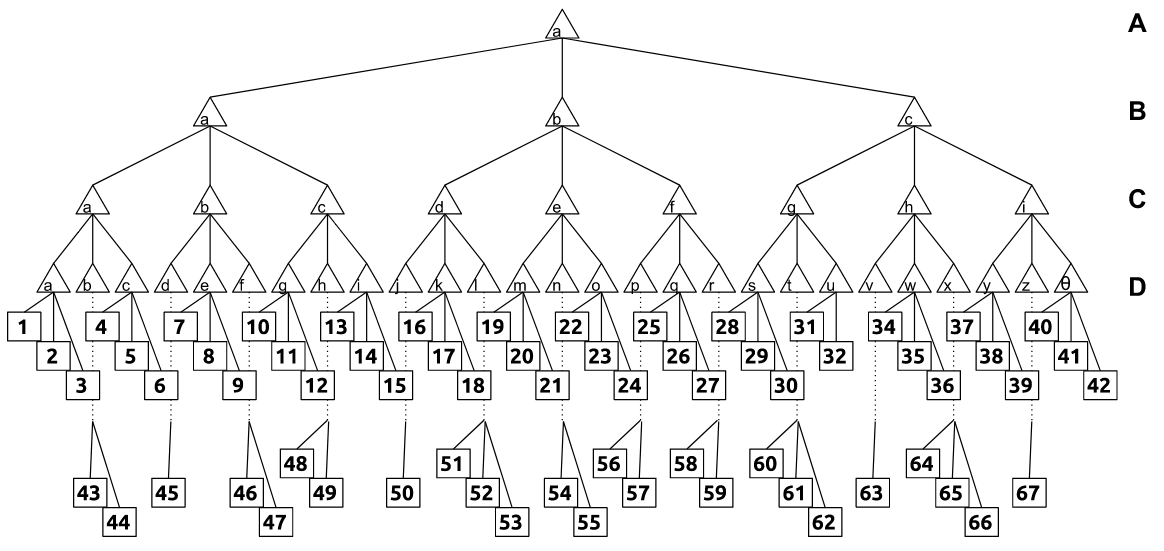
\includegraphics[width=\textwidth]{Images/game_tree.png}

\rule{\textwidth}{0.5pt}

\section*{2. Zero-sum Game Tree}
(25 pt) Below is a 2 player zero-sum game tree. Solve the game tree using
    minimax with alpha beta pruning. Show your work.

\rule{\textwidth}{0.5pt}

\section*{3. Zero-sum Game Tree}
(25pt) Below is a 2 player zero-sum game with chance nodes. Solve the game tree
    using expectiminimax and no pruning. Show your work

\rule{\textwidth}{0.5pt}

\section*{4. Nash Equilibrium}
(25pt) Find the Nash Equilibrium(s) of the below normal form games. Show your
    work

\begin{enumerate}[label=\alph*.]
    \item (5 pt)
    \item (5 pt)
    \item (5 pt) Hint: If you cannot apply the algorithm, check each state
        manually for being a Nash Equilibrium
    \item (10 pt)
\end{enumerate}

\end{flushleft}
\end{document}
